%%%%%%%%%%%%%%%%%%%%%%%%%%%%%%%%%%%%%%%%%
% FRI Data Science_report LaTeX Template
% Version 1.0 (28/1/2020)
%
% Jure Demšar (jure.demsar@fri.uni-lj.si)
%
% Based on MicromouseSymp article template by:
% Mathias Legrand (legrand.mathias@gmail.com)
% With extensive modifications by:
% Antonio Valente (antonio.luis.valente@gmail.com)
%
% License:
% CC BY-NC-SA 3.0 (http://creativecommons.org/licenses/by-nc-sa/3.0/)
%
%%%%%%%%%%%%%%%%%%%%%%%%%%%%%%%%%%%%%%%%%


%----------------------------------------------------------------------------------------
%	PACKAGES AND OTHER DOCUMENT CONFIGURATIONS
%----------------------------------------------------------------------------------------
\documentclass[fleqn,moreauthors,10pt]{ds_report}
\usepackage[english]{babel}
\usepackage[section]{placeins}
\graphicspath{{fig/}}
\usepackage{float}



%----------------------------------------------------------------------------------------
%	ARTICLE INFORMATION
%----------------------------------------------------------------------------------------

% Header
\JournalInfo{UL FRI Data Science - Introduction to Data Science, 2021-2022}

% Interim or final report
%\Archive{Interim report}
\Archive{Project 3 Report}

% Article title
\PaperTitle{How bad could a single feature be?
}

% Authors and their info
\Authors{Vito Založnik\textsuperscript{1}}
\affiliation{\textsuperscript{1}\textit{vz9592@student.uni-lj.si, 63210496}}

% Multiple authors
%\Authors{John Doe\textsuperscript{1}, Jane Doe\textsuperscript{2}, and Mike Smith\textsuperscript{3}}
%\affiliation{\textsuperscript{1}\textit{john.doe@fri.uni-lj.si, 63181234}}
%\affiliation{\textsuperscript{1}\textit{jane.doe@fri.uni-lj.si, 63185678}}
%\affiliation{\textsuperscript{1}\textit{mike.smith@fri.uni-lj.si, 63171234}}

% Keywords
\Keywords{Predictive modeling, Feature importance, Paying, Cancelled}
\newcommand{\keywordname}{Keywords}


%----------------------------------------------------------------------------------------
%	ABSTRACT
%----------------------------------------------------------------------------------------

\Abstract{ In this report, I wanted to find answers to two questions. Can we find out if the paying company will stop paying and if the non-paying company will start to pay?  Such answers could help Databox plan future upgrades on their platform. In each problem, I also wanted to find features with the biggest impact on made decisions. I evaluated models with an Accuracy score and F1 score and they seem suitable to answer those questions. I feel that more events data could make models even better. An important side observation was, that a $query\_builder$ trial feature is so bad, that is deterring customers from subscribing instead of convincing them. 

}

%----------------------------------------------------------------------------------------

\begin{document}

% Makes all text pages the same height
\flushbottom

% Print the title and abstract box
\maketitle

% Removes page numbering from the first page
\thispagestyle{empty}

%----------------------------------------------------------------------------------------
%	ARTICLE CONTENTS
%----------------------------------------------------------------------------------------

\section*{Introduction} 
	Predictive modeling is a commonly used statistical technique to predict future behavior. Predictive modeling solutions are a form of data-mining technology that works by analyzing historical and current data and generating a model to help predict future outcomes. In predictive modeling, data is collected, a statistical model is formulated, predictions are made, and the model is validated (or revised) as additional data becomes available.
	
Databox company provided us an anonymized and sampled dataset on their platform usage data from the last 2 years.
 Data were combined
from file with signups attributes and files with events. Our task was to select a few problems and predict outcomes. For the first problem, I decided to try to build a model for the prediction of already paying companies to cancel their subscription.  For the second problem, I decided to try to build a model for the prediction of a company to start paying and to explore feature importance. 


%------------------------------------------------

\section*{Methods}

\subsection*{Data preprocessing}
First, I had to join together all events and signups tables. The problem was, that IDs in the signup table and all events tables were chosen randomly and there were not enough equal IDs in all tables to use inner join. So I decided to use outer join and replace all missing values with 0. Then I changed string boolean values to numerical and decompose $trial\_features$ columns into indicating columns of each of the trial features. This was used as a base dataset and was later modified for each problem as needed. In the case of both problems, I used simple random sampling to resample my data set in such a way that the data was not imbalanced anymore.

\subsection*{Algorithms}

Both problems are classification problems so I decided to use some most well-known classification algorithms. 
Algorithms used were:
\begin{itemize}
    \item Suport Vector Machine
    \item K Nearest Neighbours
    \item Random Forest
    \item Naive Bayes
\end{itemize}
With each algorithm and problem, I tried to find the best possible parameters. 

\subsection*{Scoring}

To evaluate all the models I used 10-fold cross-validation. Since the dataset were balanced, I decided to use an accuracy score as the main scoring function for both problems. The basic score with random guessing would be $ 50 \% $, so any useful algorithm should get an accuracy score of at least $ 50 \% $. I also calculated the F1 score as it is the weighted average of Precision and Recall. 

\section{From paying to cancelling}
As the first problem, I wanted to answer the question of whether it is possible to predict whether a paying company will cancel a subscription and what are the main reasons for this.

\subsection{Data preprocessing}
From my base dataset, described in $Methods$ I removed $Country$ column and used only rows with companies that at some point started the subscription. I also added a column called $days\_since\_paying$. In this column were integers representing days between the time of the creation of the company and the start of the subscription. In the remaining dataset were 1156 companies that canceled subscriptions and 1794 that did not. With simple random sampling, I choose 1156 of not canceled so the dataset was balanced. Then I scaled all the data  between $0$ and $1$ using $MinMaxScaler$.Since there were so many problems with missing events data, I tried to run all algorithms on data with events columns and also on data without events columns. The results were still better, even with a small number of events.    

\subsection{Models}
I trained four different models on various different parameters to find the best possible one. All models were used from $sklearn$ library. SVM algorithm used kernel $linear$. KNN gave best results with $k=33$. Random Forest used $26$ decision trees in forest. For Naive Bayes I choose $GausianNB$ algorithm.

\subsection{Evaluation and feature imnportance}
We evaluated our models with a 10-fold cross-validation and accuracy score as the main scoring function. Since this was a binary classification problem the base score obtained with random guessing was $50\%$.


\begin{figure}[h]\centering
	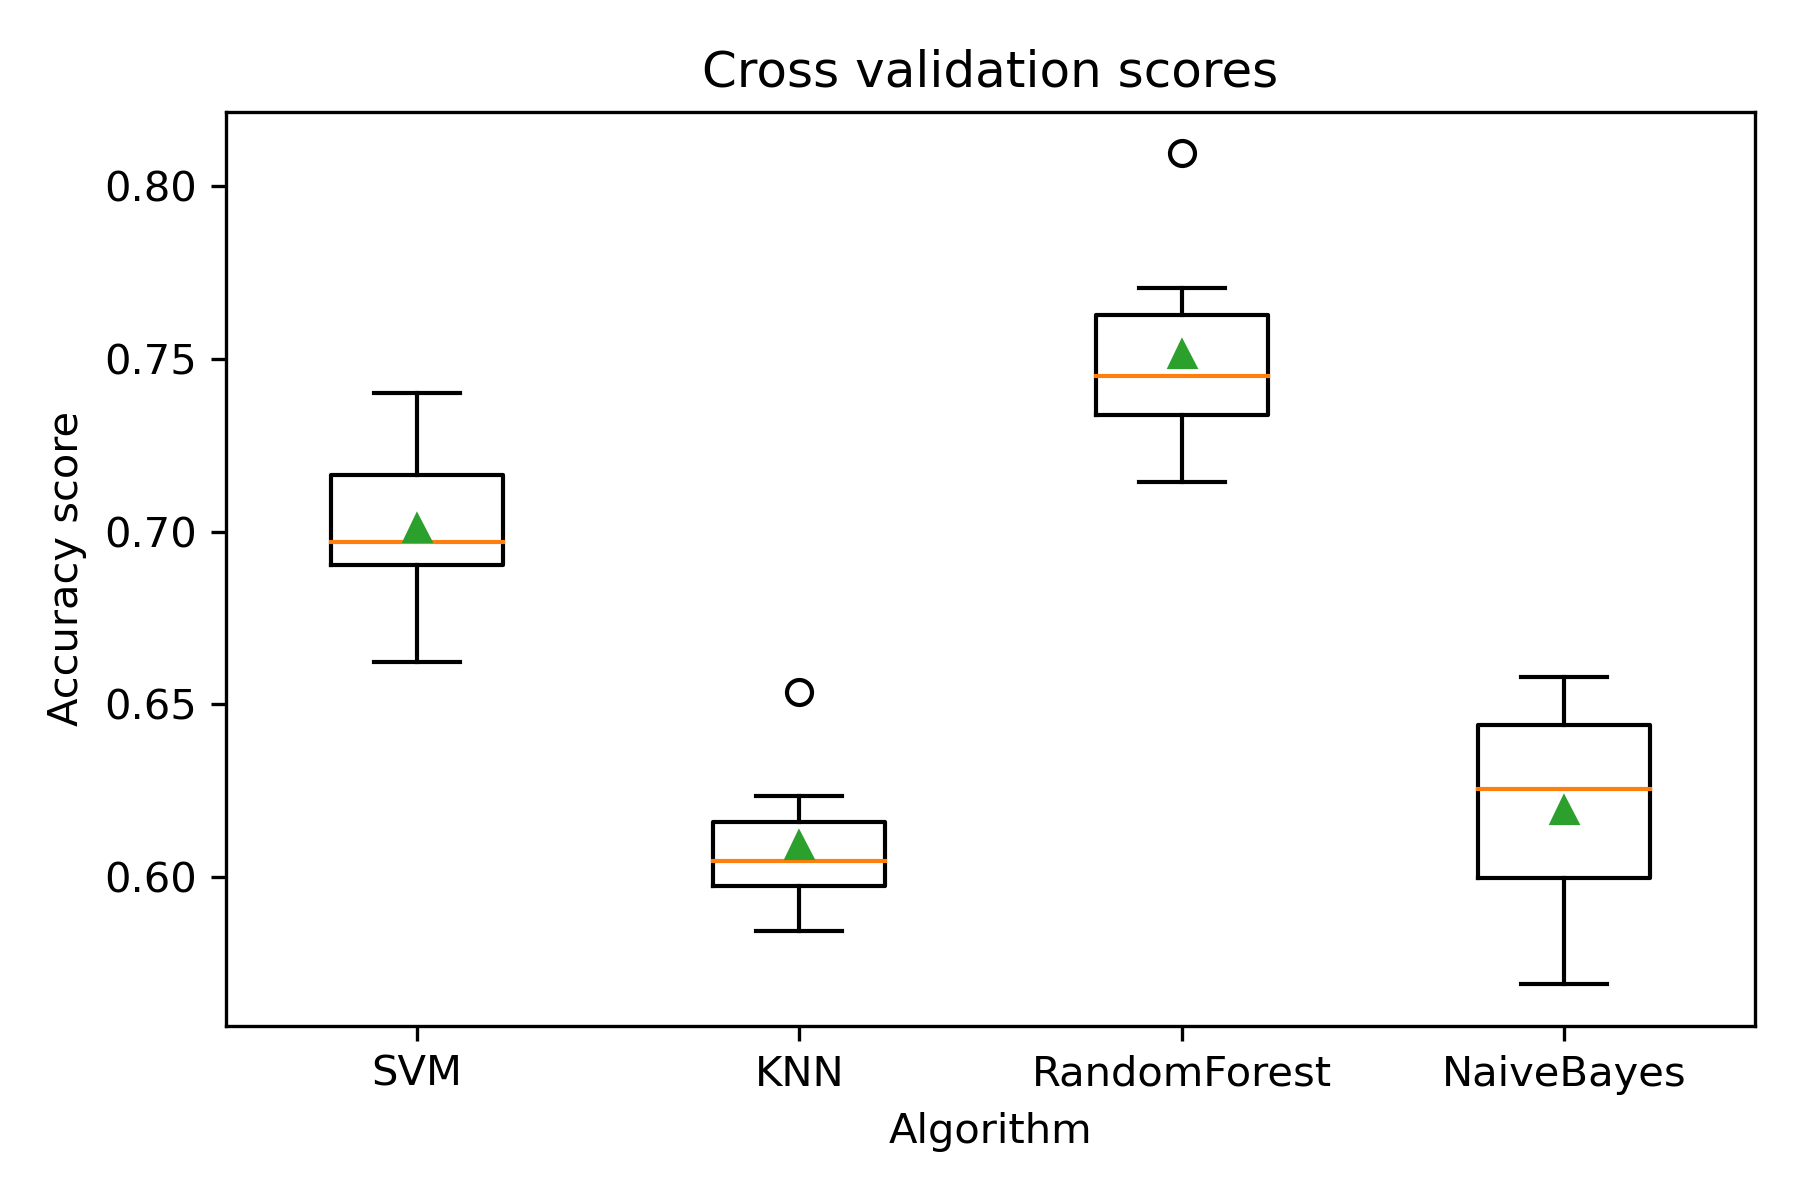
\includegraphics[width=\linewidth, height=7cm]{problem_1_boxplot.png}
	
	\caption{\textbf{Boxplots of cross validation scores.} We can see, that the best performing algorithms were SVM and Random Forest. Naive Bayes and KNN were slightly worse. All of the algorithms outperformed the base score.  The green triangle represents the mean and the yellow line represents the median. }
	\label{boxplot1}
\end{figure}


\begin{center}
\begin{table}
\caption{\label{table_1} Mean of scores.}

\begin{tabular}{|c|| c| c| c| c|} 
 \hline
 Scoring  & SVM & KNN & Randomorest  & NaiveBayes\\ 
 \hline\hline
 Accuracy & 0.707 & 0.618 &  0.745 & 0.626\\ 
 \hline
 F1 & 0.743 & 0.628 & 0.731 & 0.697 \\
 \hline
\end{tabular}
\end{table}
\end{center}

In Figure \ref{boxplot1} We can see, that the highest average accuracy score was obtained using the Random Forest algorithm. In table \ref{table_1} are all mean accuracy and F1 scores obtained. Since this was binary classification problem, I would choose SVM as the main model even if the scores are a little lower. Random Forest is too much of a black box kind of algorithm and is very difficult to figure out feature importance from it. It is also harder to tune it due to its complexity.  On the other side, SVM has a very clear overview of which features are pointing to one side of the hyperplane and which to the other.

\begin{figure}[h]\centering
	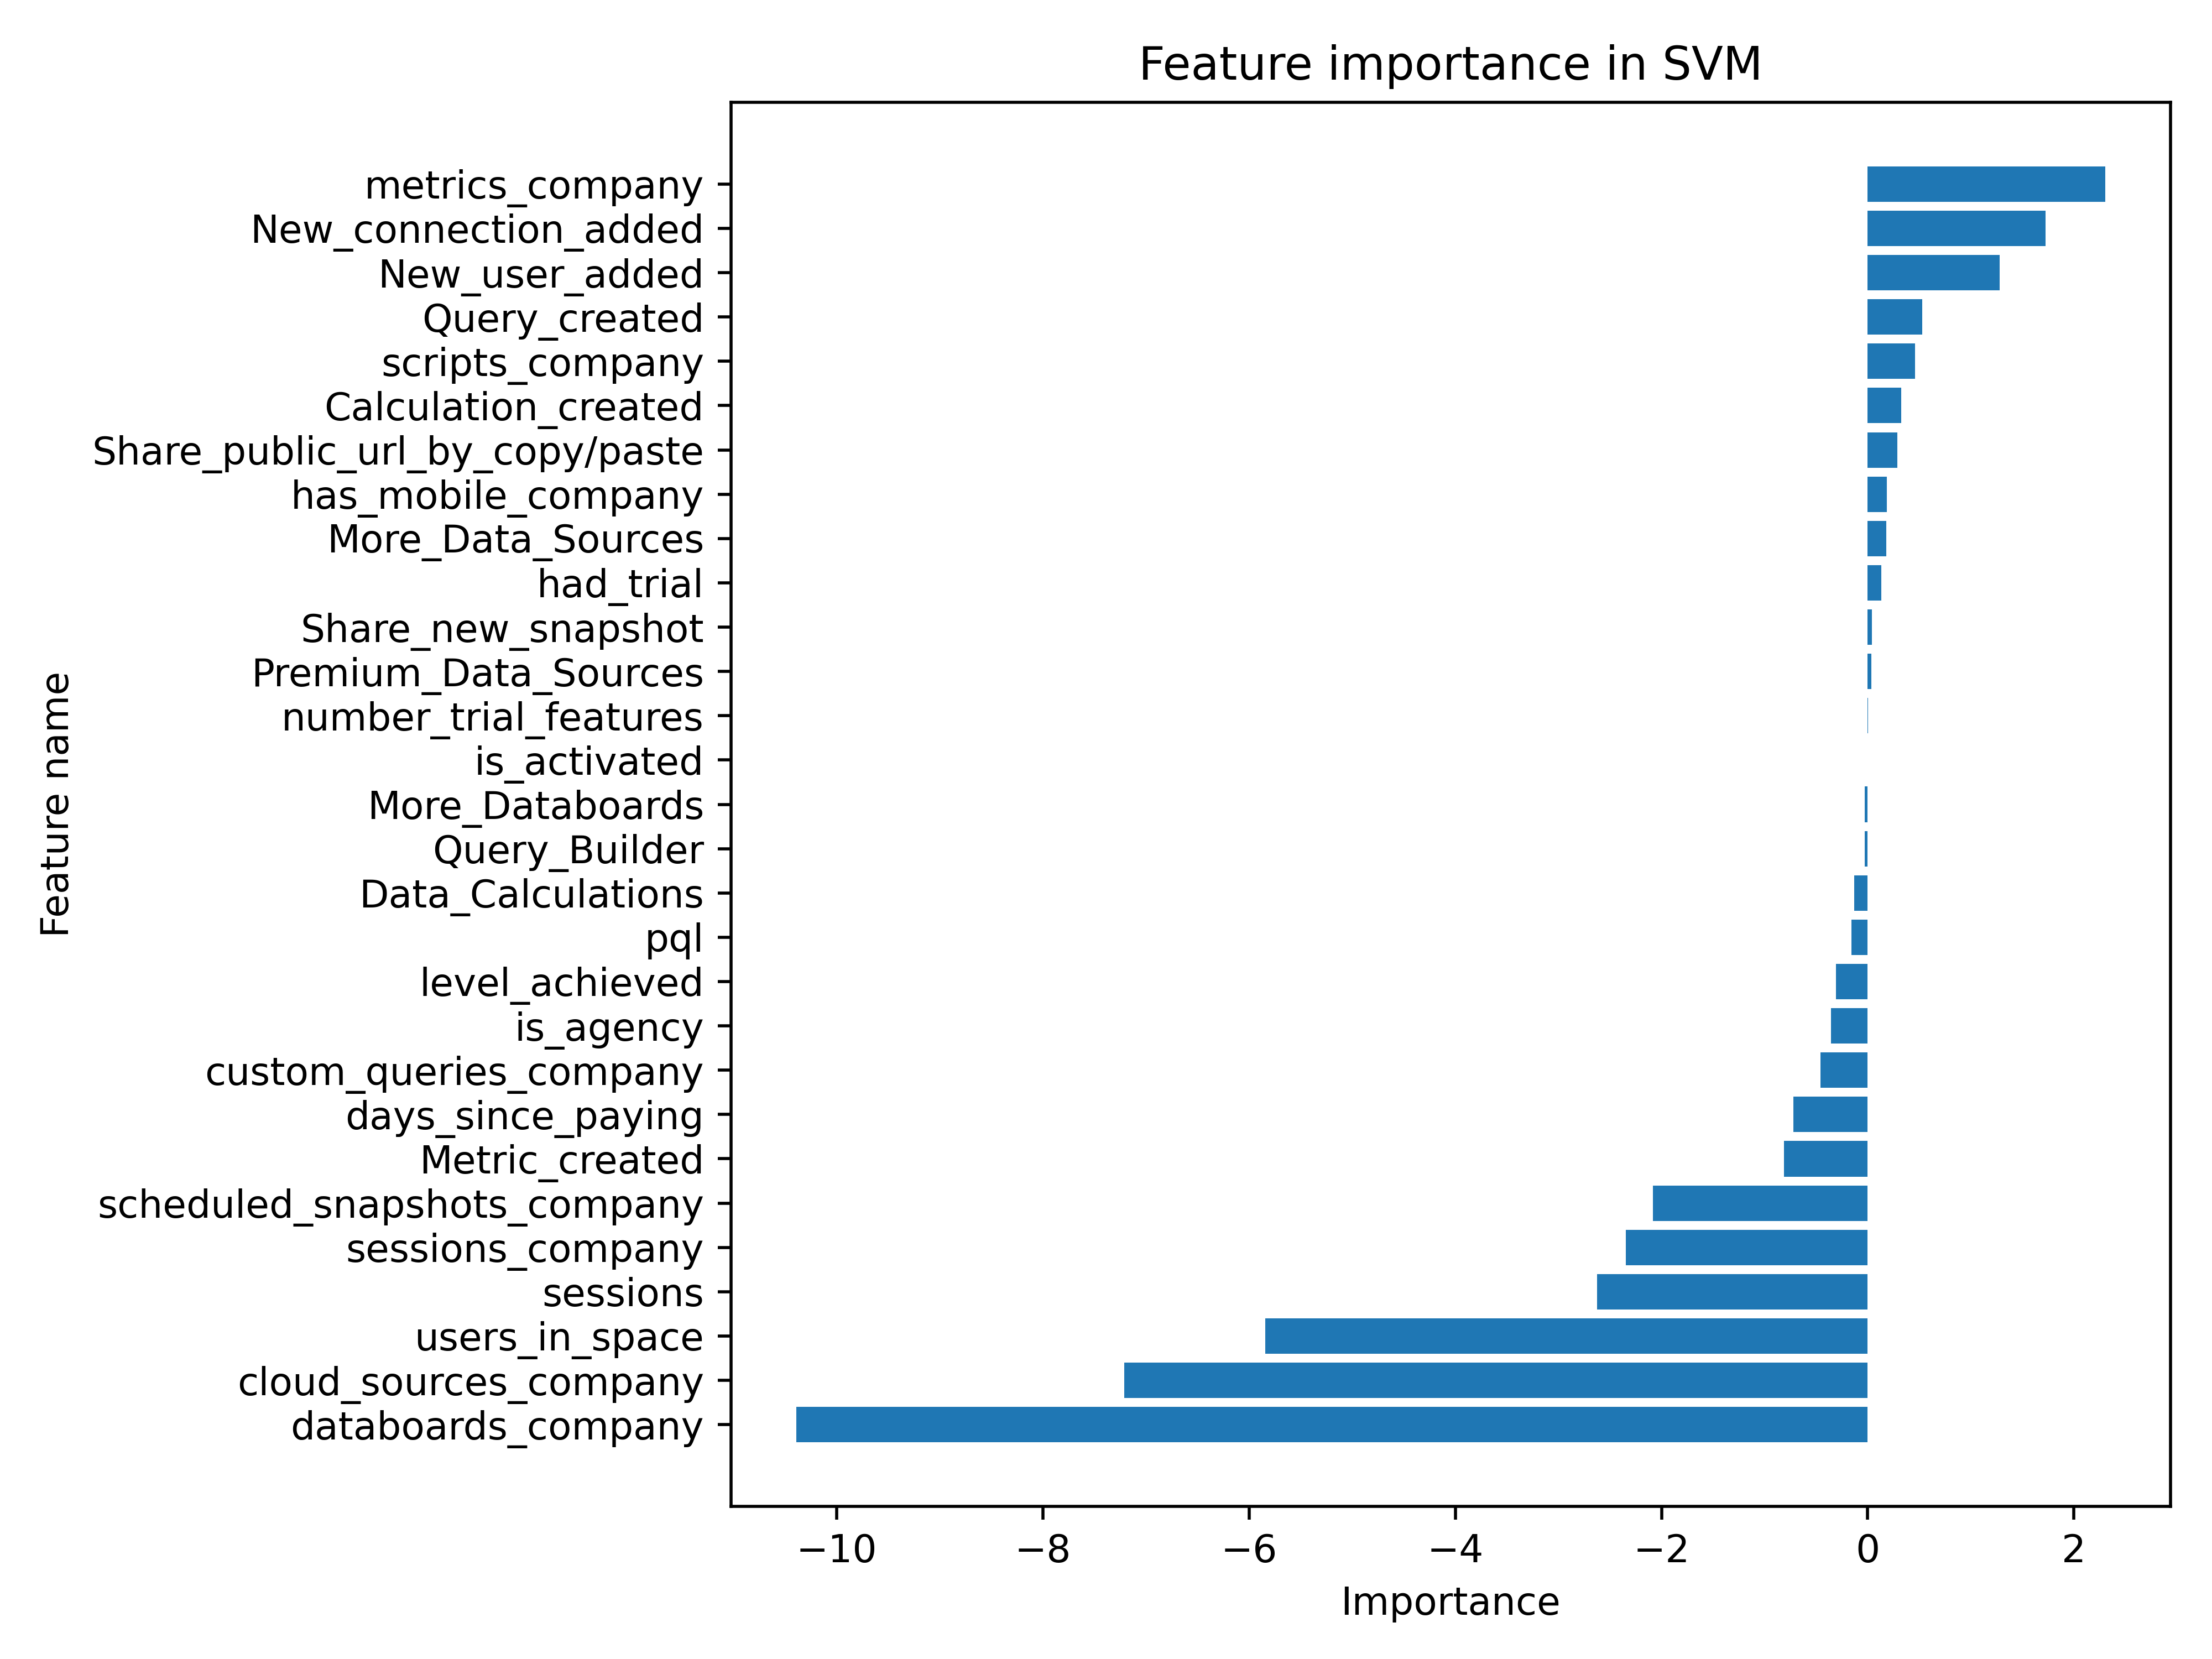
\includegraphics[width=\linewidth, height=10cm]{SVM_feature_imp.png}
	
	\caption{\textbf{Barchart of feature importance.}}
	\label{feature_importance_1}
\end{figure}

In Figure \ref{feature_importance_1} we can see, that by far the most important features in deciding if a customer will stop paying are $databoards\_company$, $cloud\_sources\_company$ and $users\_in\_space$. It is interesting, that even with low frequency of events data, $sessions$ are among most important features.

Models made a big improvement compared to base score of $50\%$. They are not perfect, but can still be a good estimators. 


\section{From non-paying to paying}
For the second problem I wanted to see if it is possible to predict which companies will start paying for Databoxs services. 

\subsection{Data preprocessing}
First I filtered the dataset and kept only the ones with an activated account. The purpose of this was to clean the data from those who came only once to see the page. This split dataset almost in half. Then I dropped $pql$ columns since I did not want to "cheat" and use an already made estimator from Databox. I also dropped columns $cancelled$ since this was a clear indicator that the company has been paying in the past. I considered using one-hot encoding to transform categorical column $country$ into numerical but decided to drop it instead. After all this filtering there were 49869 non-paying companies and  2933 paying companies. I considered filtering the data, even more, on only those who used the trial. This would reduce non-paying to 12772 and keep almost all paying with 2792. But later, while training models on both possible versions, it showed that $had\_trial$ feature was one of the best indicators, so I decided to keep it. Then I used simple random sampling to randomly choose 2792 non-paying companies that, together with 2792 paying. This formed a final dataset. Then I scaled the data with $MinmaxScaler$ such that all the values were between $0$ and $1$.



\subsection{Models}
As in problem 1, I trained all four models with several different parameters. SVM algorithm used kernel $linear$. KNN gave best results with $k=5$. Random Forest used $48$ decision trees in forest. For Naive Bayes I choose $GausianNB$ algorithm.


\subsection{Evaluation and feature importance}
As in problem 1 I used 10-fold cross-validation to validate models. Since the dataset was balanced, the base accuracy score was $50\%$. 



\begin{figure}[h]\centering
	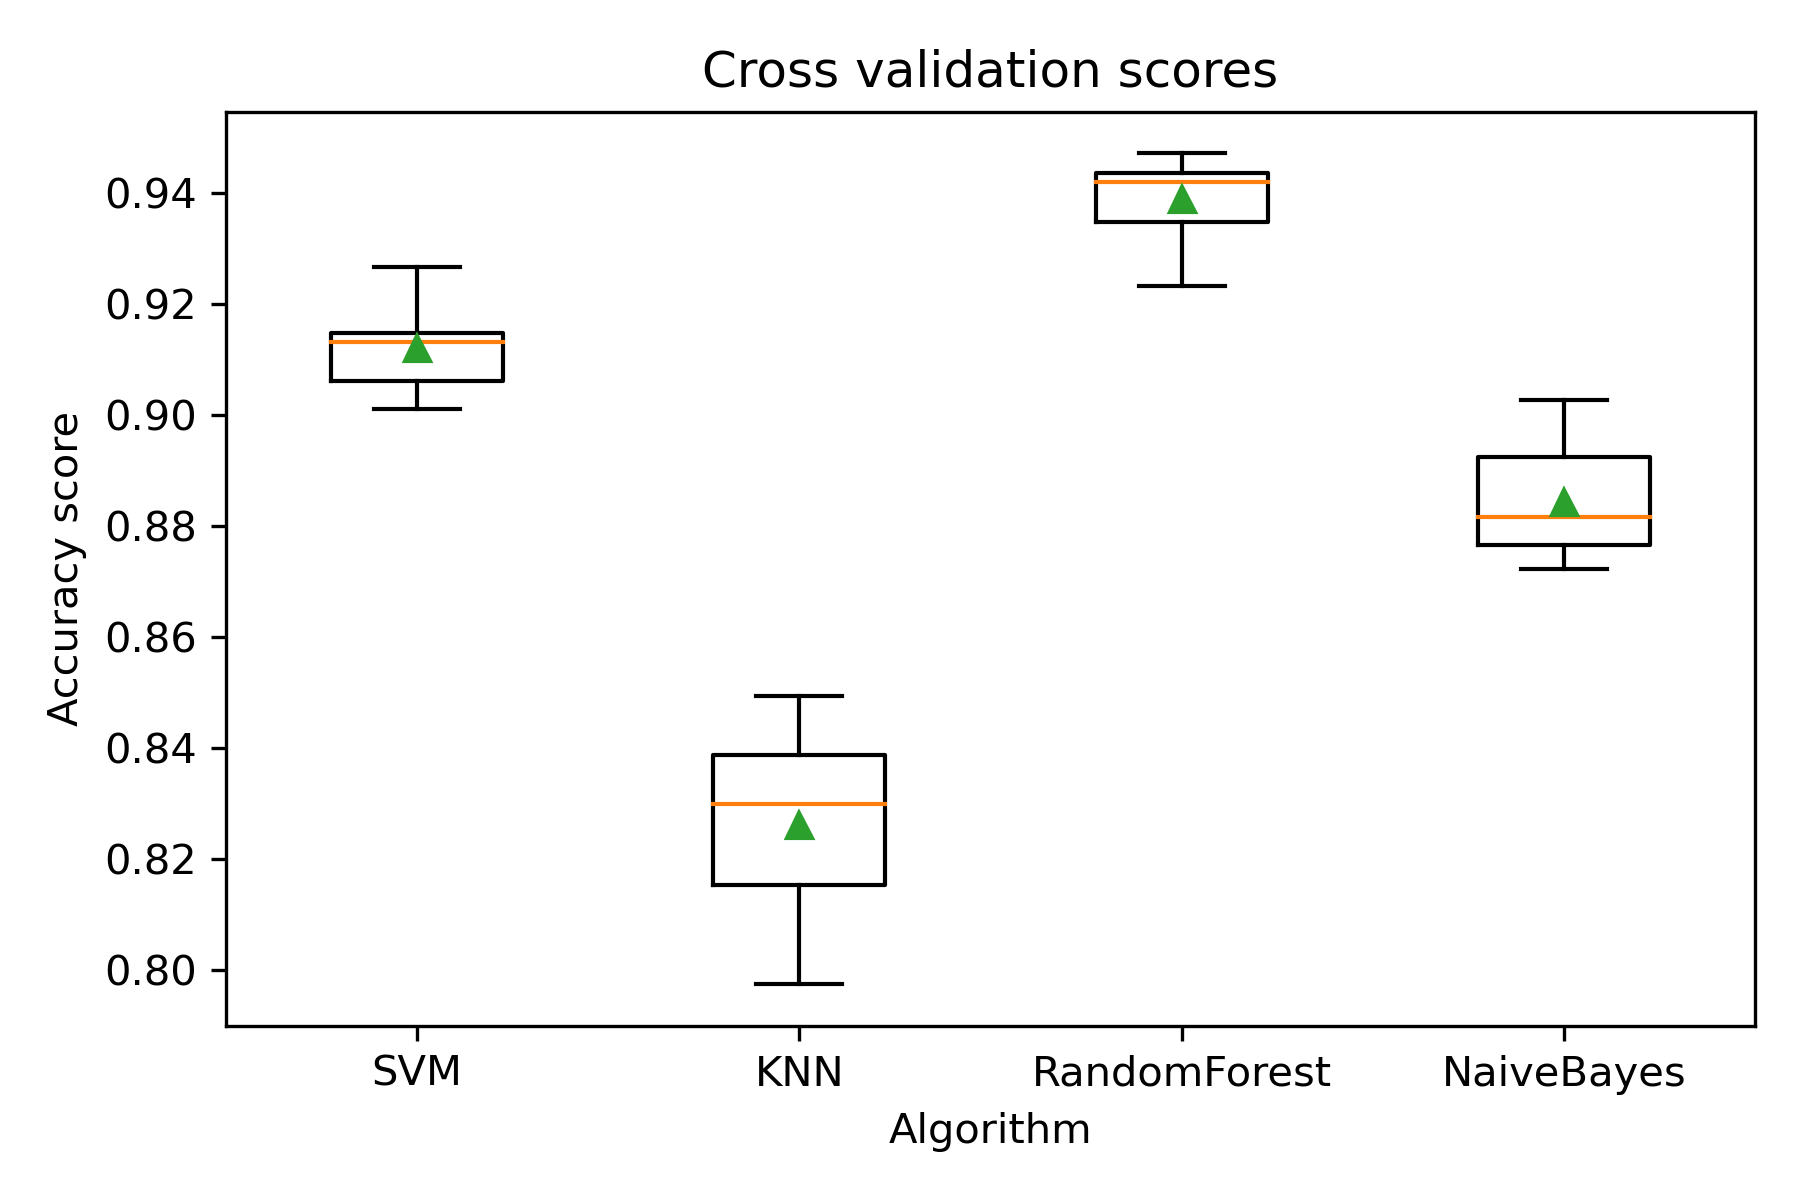
\includegraphics[width=\linewidth, height=7cm]{problem_2_boxplot_all_data.png}
	
	\caption{\textbf{Boxplots of cross validation scores.} We can see, that again, Random Forest and SVM gave the best results. But in this Naive Bayes and even KNN gave pretty good results. All were far above a base score of $50\%$ and in the case of Random Forest and SVM even above $90\%$.Yellow line is median and green triangle is mean. }
	\label{boxplot2}
\end{figure}

In Figure \ref{feature_importance_2} we can see that the most important features in predicting if a company will start to pay or not. Those are $sessions\_company$, $new\_conenction\_added$,$\cdots$  But the most interesting is, that $Query\_Builder$, a trial feature, that should convince potential subscribers to subscribe after the trial ends, is doing exactly the opposite.  It is showing towards the half of hyperplane that is indicating that company will not start paying.

I think that the results are good enough to use both SVM and Random Forest as competent validators. Also variances between cross validations were relatively small. Also Naive Bayes seems like quite a good option, but I would not use it because it assumes that the features are independent, but in practice they are not. 


\begin{center}
\begin{table}
\caption{\label{table_2} Mean of scores.}

\begin{tabular}{|c|| c| c| c| c|} 
 \hline
 Scoring  & SVM & KNN & RandomForest  & NaiveBayes\\ 
 \hline\hline
 Accuracy & 0.912 & 0.826 &  0.939 & 0.884\\ 
 \hline
 F1 & 0.913 & 0.899 & 0.935 & 0.874 \\
 \hline
\end{tabular}
\end{table}
\end{center}





\begin{figure}[h]\centering
	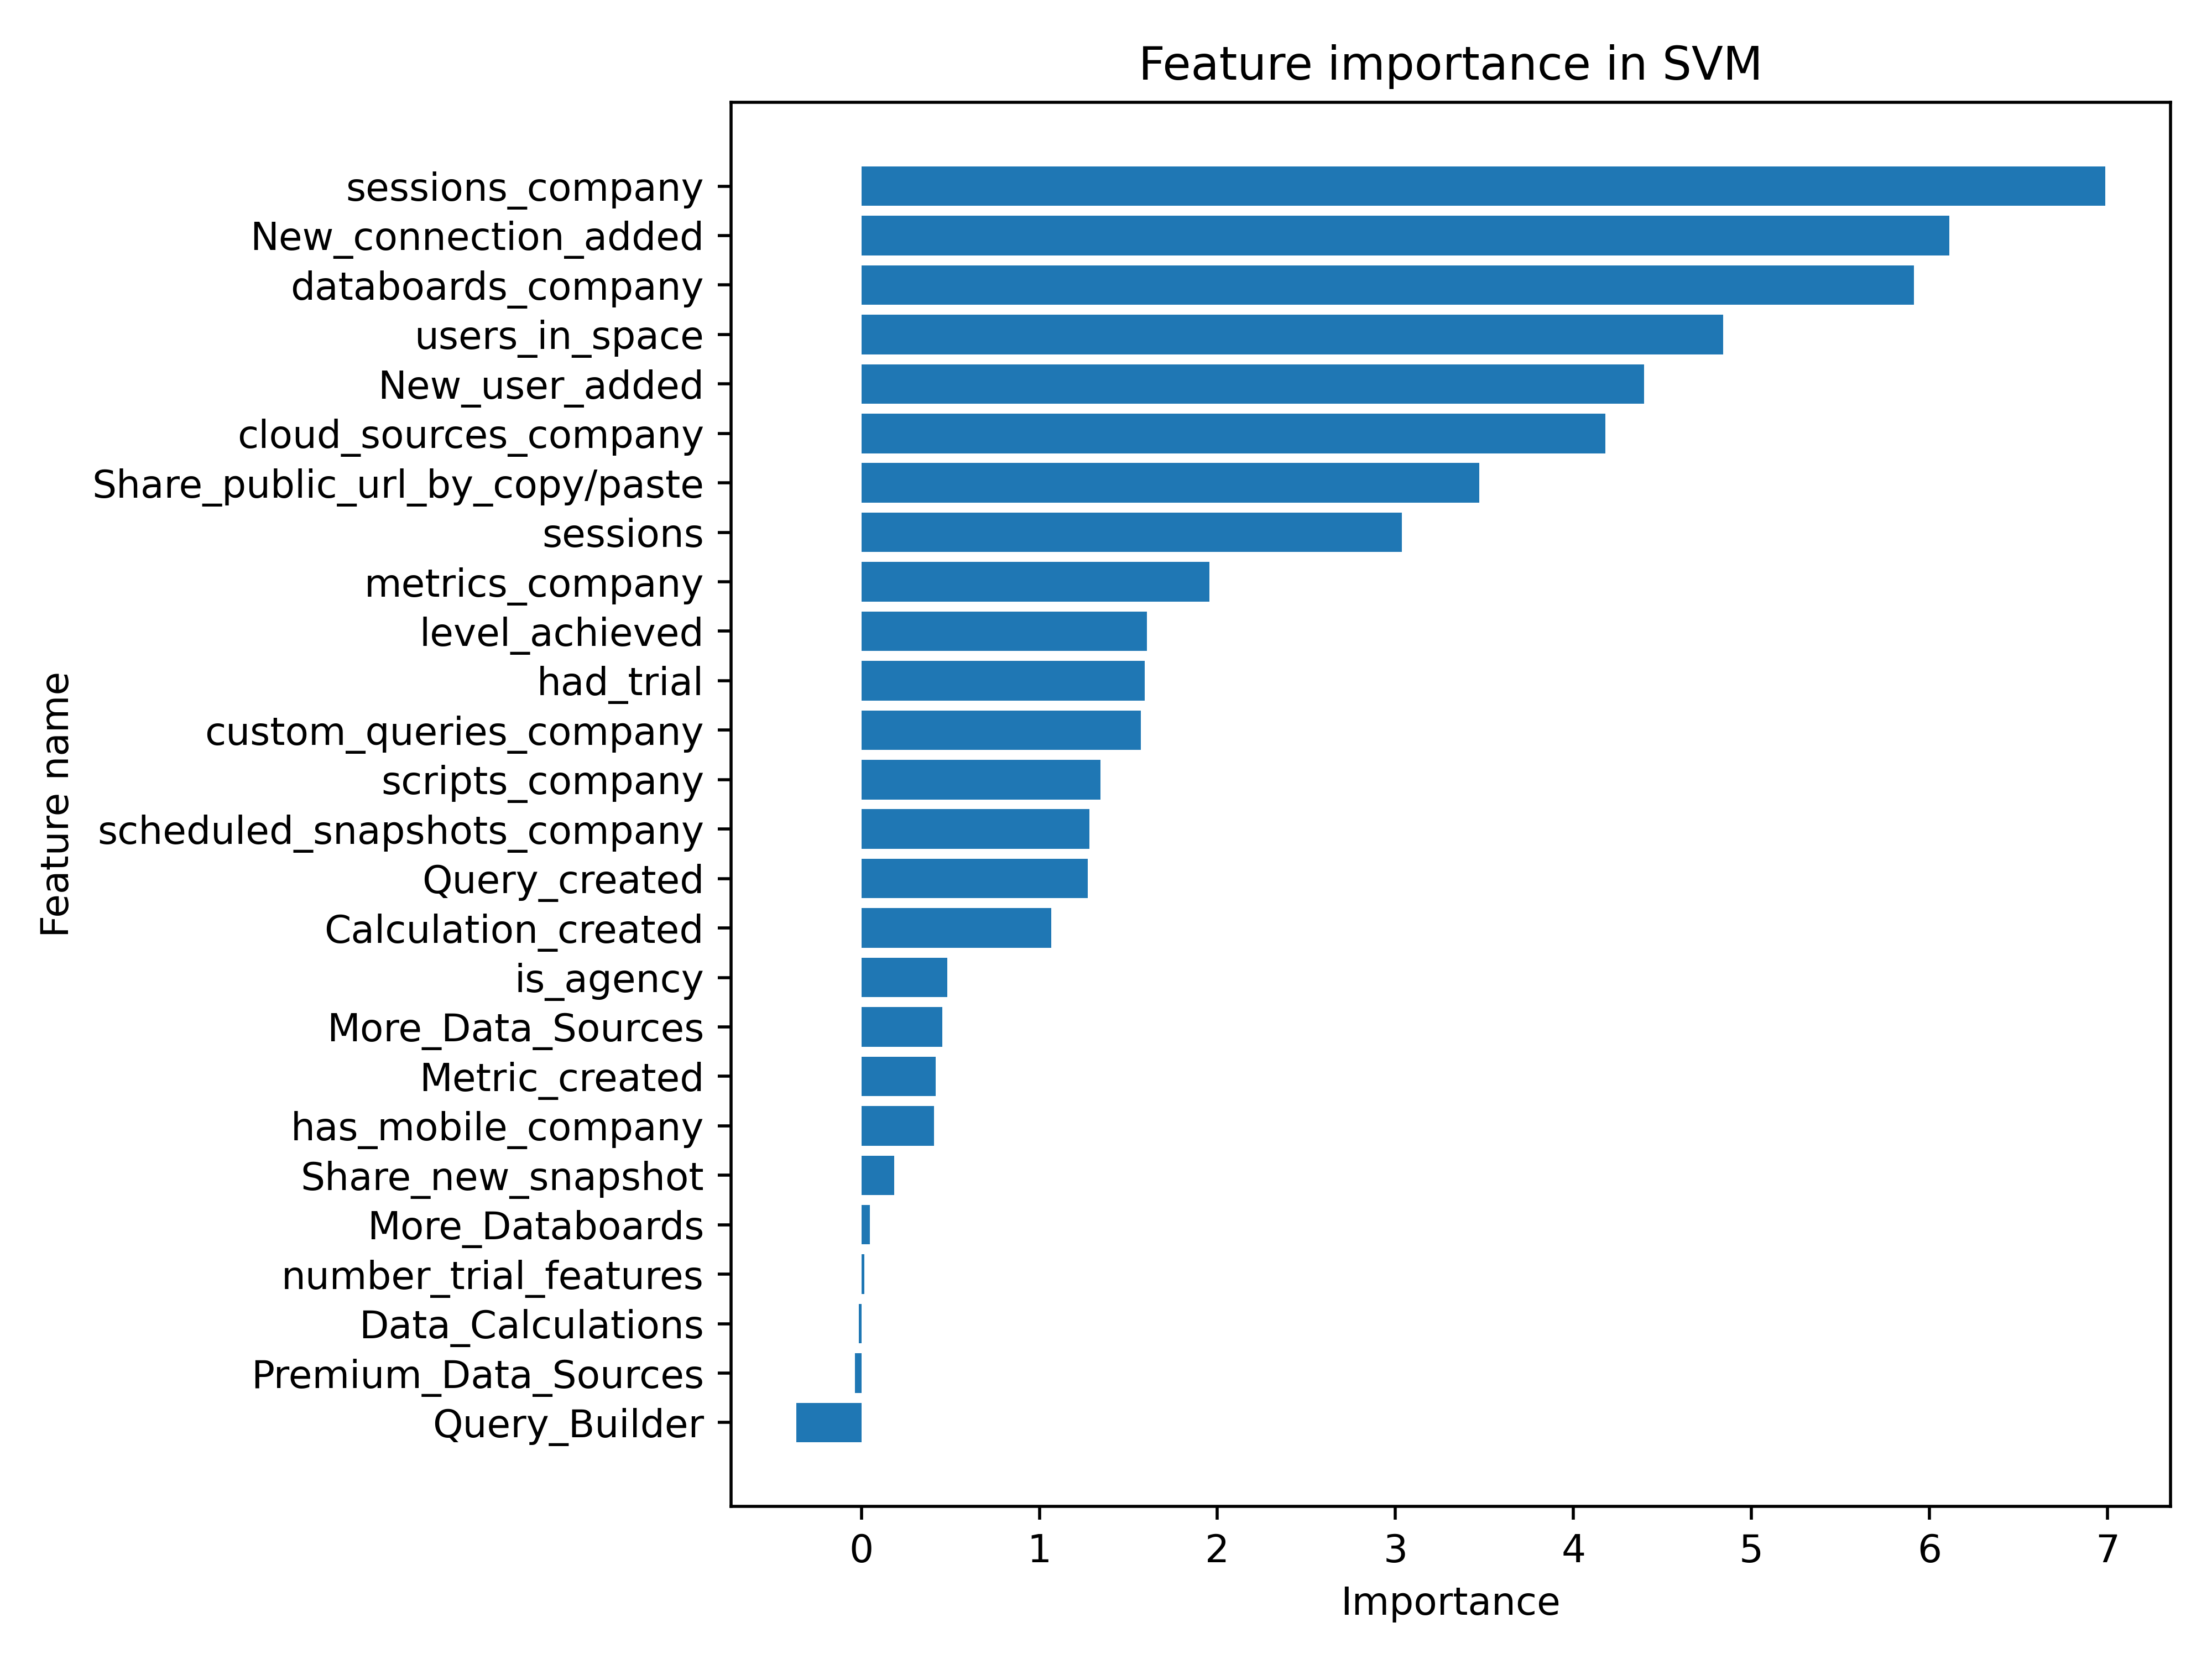
\includegraphics[width=\linewidth, height=8cm]{SVM_feature_imp_all_data.png}
	
	\caption{\textbf{Barchart of feature importance.}}
	\label{feature_importance_2}
\end{figure}
%------------------------------------------------

\section*{Discussion}
In this report, I analyzed the data of Databox's platform usage. I tried to build models that could predict if a paying company will stop paying and if a non-paying company will start paying. Obtained results were good enough to use it. Problem 1 model was correct in around $70\%$ and problem 2 models were correct in more than $90\%$. It is bad that there was not enough consistency in sampling event data so we could have more companies with data for all events. This could help to improve our models as some of the events showed to be one of the most important features.


Databox should also reconsider their $query\_builder$ feature as it seems that is doing exactly the opposite as it should. Instead of convincing non-paying companies to subscribe, is actually deterring them from doing so. 





\end{document}
